\documentclass{article}
\usepackage[utf8]{inputenc}
\usepackage{minted}
\usepackage{amsmath}
\usepackage{vmargin}
\usepackage{times}
\usepackage{subfigure}
\usepackage{graphicx}
\usepackage{hyperref}
\hypersetup{
    colorlinks=true,
    linkcolor=blue,
    filecolor=magenta,      
    urlcolor=cyan,
}
 
\urlstyle{same}

\usepackage{color}
\definecolor{gray97}{gray}{.97}
\definecolor{gray75}{gray}{.75}
\definecolor{gray45}{gray}{.45}

\usepackage{listings}
\lstset{ frame=Ltb,
framerule=0pt,
aboveskip=0.5cm,
framextopmargin=3pt,
framexbottommargin=3pt,
framexleftmargin=0.4cm,
framesep=0pt,
rulesep=.4pt,
backgroundcolor=\color{gray97},
rulesepcolor=\color{black},
%
stringstyle=\ttfamily,
showstringspaces = false,
basicstyle=\small\ttfamily,
commentstyle=\color{gray45},
keywordstyle=\bfseries,
%
numbers=left,
numbersep=15pt,
numberstyle=\tiny,
numberfirstline = false,
breaklines=true,
}

% minimizar fragmentado de listados
\lstnewenvironment{listing}[1][]
{\lstset{#1}\pagebreak[0]}{\pagebreak[0]}

\lstdefinestyle{consola}
{basicstyle=\scriptsize\bf\ttfamily,
backgroundcolor=\color{gray75},
}

\lstdefinestyle{C}
{language=C,
}

\title{Escalona\_Joaquin\_5}
\date{September 2018}

\setpapersize{A4}
\setmargins{2.5cm}       % margen izquierdo
{1.5cm}                        % margen superior
{16.5cm}                      % anchura del texto
{23.42cm}                    % altura del texto
{10pt}                           % altura de los encabezados
{1cm}                           % espacio entre el texto y los encabezados
{0pt}                             % altura del pie de página
{2cm}                           % espacio entre el texto y el pie de página


%-------------------------------------------------------------------------%
\begin{document}

\maketitle

%-------------------------------------------------------------------------%
\section{Ejercicio 1}
 El método Newton requiere
conocimiento de la derivativa de $f(x)$, $f'(x)$, y que esta no sea igual a 0. Hay instancias en que
estas condiciones no se cumplen. Por ejemplo, es posible que tengamos una función en
forma de una tabla discreta. O a veces, la derivativa $f'(x)$ puede ser una expresión muy
complicada, y puede ser poco práctico calcularla de forma analítica. En estos casos, podemos
usar el método del secante, un método que es 3000 años más antiguo que el método de
Newton. Con este método, no usamos la derivativa $f'(x)$, pero vamos a aproximarlo con la
diferencia entre dos puntos. Suponga que tenemos dos supuestos $x_n$ y $x_{n-1} $ del cero de la
función. Entonces, podemos aproximar la derivativa como
\begin{equation*}
    f'(x) = \frac{f(x_n)-f(x_{n-1})}{x_n - x_{n-1}}
\end{equation*}
Con esta aproximación, un supuesto mejor es
\begin{equation*}
    x_{n+1} = x_n - f(x_n)\frac{x_n - x_{n-1}}{f(x_n)-f(x_{n-1})}
\end{equation*}
a) Implemente este método para determinar la raíz de las siguientes funciones:

\begin{enumerate}
    \item $f(x) = x^3 - 5$
    \item $f(x) = x^{3/5}-16$
    \item $f(x) = cos(x) - 6x$
\end{enumerate}
\subsection{Solución apartado A} 
    Código python \href{https://github.com/joescalona/Programacion-Astronomica/blob/master/Tarea\%205/problema1_A.py}{aquí}
    \begin{minted}{python}
    #-*- coding:utf-8 -*-
    
    #https://www.uv.es/~diaz/mn/node21.html
    
    #importamos math para el coseno
    from math import cos
    
    #definimos las funciones
    
    #f1(x) ---> x^3 - 5
    def f1(x):
    	return x**3 - 5
    
    #f2(x) --->  x^(3/5) - 16
    def f2(x):
    	return x**(3./5.) - 16
    
    #f3(x) ---> cos(x) - 6x
    def f3(x):
    	return cos(x) - 6*x
    
    #definimos la funcion "secante" para comprimir la cantidad de codigo.
    def secante(f,xi,xf):
    	"""Funcion que aproxima una raiz mediante el método de la secante. 
    	Argumentos:
    	f  = funcion a calcular su raiz
    	xi = valor inicial del intervalo
    	xf = valor final del intervalo
    	"""
    	#definimos el error tolerado
    	error = 0.001
    	#respuesta (respt) es el punto medio entre el valor inicial y el final
    	respt = (xi + xf)/2. 
    	#iteraciones
    	itera = 0
    	#generar respuesta cada vez más precisa por el método de la secante
    	while (abs(f(respt)))>0.001: 
    		respt = xf - (f(xf)*(xf -xi))/(f(xf)-f(xi))
    		itera += 1
    	#se cambian los papeles para poder continuar con el método.
    	#lo vi aquí: https://www.youtube.com/watch?v=YOHtIzPmfzE
    		xi = xf
    		xf = respt 
    	print '*** Han ocurrido',itera,'iteraciones'
    	print '*** La aproximacion final de la raiz es',respt
    print '-------- Metodo de la secante --------\n'
    #funcion f1(x)
    print 'Función => f1(x) = x^3 - 5'
    secante(f1,-10.0,10.0)
    
    #funcion f2(x)
    print '\nFunción => f2(x) = x^(3/5) - 16'
    secante(f2,50.0,200.0)
    
    #funcion f3(x)
    print '\nFunción => f3(x) = cos(x) - 6x'
    secante(f3,-10.0,10.0)
    \end{minted}
    
    \noindent
    Arroja como resultado:
    \begin{lstlisting}[style=C,numbers=none]
     -------- Metodo de la secante --------

    Funcion => f1(x) = x^3 - 5
    *** Han ocurrido 309 iteraciones
    *** La aproximacion final de la raiz es 1.7099769978

    Funcion => f2(x) = x^(3/5) - 16
    *** Han ocurrido 4 iteraciones
    *** La aproximacion final de la raiz es 101.593751278

    Funcion => f3(x) = cos(x) - 6x
    *** Han ocurrido 4 iteraciones
    *** La aproximacion final de la raiz es 0.164418799818
    \end{lstlisting}
\subsection{Solución apartado B}
Compare con el método de Newton. ¿Cuántas iteraciones necesita cada método con los ejemplos
de arriba?

Código python \href{https://github.com/joescalona/Programacion-Astronomica/blob/master/Tarea\%205/problema1_B.py}{aquí}
    \begin{minted}{python}
    #-*- coding:utf-8 -*-
    #importamos math para el coseno y el seno
    from math import cos,sin 
    #definimos funciones
    
    # f1(x)---> x^3 - 5
    # f1'(x)---> 3x^2 
    def f1(x):
        return x**3 - 5
    
    def df1(x):
        return 3*x**2
    
    # f2(x) --->  x^(3/5) - 16
    # f2'(x) ---> 3 / (5x^(2/5))
    def f2(x):
    	return x**(3./5.) - 16
    def df2(x):
    	return 3/(5*x**(2./5.))
    
    #f3(x) ---> cos(x) - 6x
    #f3'(x) ---> -sin(x) - 6
    def f3(x):
    	return cos(x) - 6*x
    
    def df3(x):
    	return -sin(x) - 6
    
    #definimos una funcion que tenga el m‚todo de newton
    def newton(f,df,xi):
    	"""Funcion que aproxima una raíz mediante el método de Newton-Raphson
    	Argumentos:
    	f  = funcion a calcular su raiz
    	df = derivada de f
    	xi = supuesto inicial
    	"""
    	xnew = [xi,]
    	erro = 0.001
    	resp = xnew[-1]
    	coun = 0
    
    	while True:
    		resp = resp - (f(resp)/df(resp))
    		xnew.append(resp)
    		coun += 1 
    		if abs(xnew[-2]-xnew[-1]) <= erro:
    			break
    	print '***Han ocurrido',coun,'iteraciones'
    	print '***La aproximacion final es',resp
    
    print '-------- Metodo de Newton --------'
    #funcion f1(x)
    print 'Función => f1(x) = x^3 - 5'
    newton(f1,df1,-10.0)
    
    #funcion f2(x)
    print '\nFunción => f2(x) = x^(3/5) - 16'
    newton(f2,df2,50.0)
    
    #funcion f3(x)
    print '\nFunción => f3(x) = cos(x) - 6x'
    newton(f3,df3,-10.0)
    \end{minted}
    \noindent
    Arroja como resultado:
    \begin{lstlisting}[style=C,numbers=none]
    -------- Metodo de Newton --------
    Funcion => f1(x) = x^3 - 5
    ***Han ocurrido 12 iteraciones
    ***La aproximacion final es 1.70997604262

    Funcion => f2(x) = x^(3/5) - 16
    ***Han ocurrido 4 iteraciones
    ***La aproximacion final es 101.593667326

    Funcion => f3(x) = cos(x) - 6x
    ***Han ocurrido 4 iteraciones
    ***La aproximacion final es 0.164418982912
    \end{lstlisting}
\textbf{Comparación:} la comparación me resulta difícil ya que el método de la secanta utiliza un intervalo, mientras que el método de Newton utiliza un supuesto inicial. Lo que hice fue darle el mismo comienzo. Los resultados son: 

\begin{table}[h]\centering
\begin{tabular}{ll}
Secante                      & Newton                      \\
$f(x) = x^3 - 5$             & $f(x) = x^3 - 5$            \\
Han ocurrido 309 iteraciones & Han ocurrido 12 iteraciones \\
                             &                             \\
$f(x) = x^{3/5}-16$          & $f(x) = x^{3/5}-16$         \\
Han ocurrido 4 iteraciones   & Han ocurrido 4 iteraciones  \\
                             &                             \\
$f(x) = cos(x) - 6x$         & $f(x) = cos(x) - 6x$        \\
Han ocurrido 4 iteraciones   & Han ocurrido 4 iteraciones 
\end{tabular}
\end{table}
\newpage 
\subsection{Solución apartado C}
Use el concepto de funciones en Python para escribir una función que calcula la tercera raíz
de un número del tipo float x con una precisión $\epsilon$. x y $\epsilon$ sean parámetros formales de la
función. Use el método de Newton o de la secante dentro de la función. Repite el concepto de variables locales con este programa.

Código python \href{https://github.com/joescalona/Programacion-Astronomica/blob/master/Tarea\%205/problema1_C.py}{aquí}
    \begin{minted}{python}
    #-*-coding: utf-8

    #se define raíz cubica
    def raiz_cubica(x,e):
    	"""Funcion que calcula la raíz cúbica de un numero float usando el método de Newton-Raphson.
    	Argumentos:
    	x = valor al cual se le aplicará la raiz cúbica
    	e = error (epsilon)
    	"""
    #respuesta 
    	respt = x/2.0
    	while abs(respt**3 - x) >= e:
    #metodo de newton
    		respt = respt - (((respt**3) - x) / (3*(respt**2)))
    	print '*** La raiz de', x, 'es aproximadamente', respt
    
    print '-------- Raíz cúbica --------\n'
    numero  = float(raw_input('Ingresa un número = '))
    epsilon = float(raw_input('Ingresa el error tolerado (positivo) = '))
    while not (epsilon)>=0:
    	epsilon = float(raw_input('el error debe ser positivo! = '))
    
    raiz_cubica(numero,epsilon) 
    \end{minted}
%-------------------------------------------------------------------------%


%-------------------------------------------------------------------------%
%-------------------------------------------------------------------------%

%-------------------------------------------------------------------------%
\section{Ejercicio 2}
Escriban dos funciones para calcular el factorial de un numero X entero y positivo, una función debe ser recursiva y la otra iterativa. Midan cual es la función mas rápida de ejecutar con un programa que compare los dos métodos.

\subsection{Factorial (Iterativo)}
Código python \href{https://github.com/joescalona/Programacion-Astronomica/blob/master/Tarea\%205/problema2_iteracion.py}{aquí}
    \begin{minted}{python}
    #-*-coding:utf-8-*-

    #Factorial Iterativo
    def factorial_iterativo(n):
    '''Función que recibe un número n y retorna n!
    '''
    mul = 1 #primera multiplicación de la iteración
    for i in range(1,n+1): #itera hasta n
        mul = mul * i #1*2*3*4*..*n
    return mul

    print '****** FACTORIAL DE UN NUMERO ******'
    
    num = abs(int(input('Número (se considerará parte entera y el valor absoluto) = ')))
    
    print 'El factorial de',num,'es',factorial_iterativo(num)
    \end{minted}
    
    \noindent
    Ejemplo para \textbf{num = 4} el programa arroja:
    \begin{lstlisting}[style=C,numbers=none]
    El factorial de 4 es 24
    \end{lstlisting}

\subsection{Factorial (Recursivo)}
Código python \href{https://github.com/joescalona/Programacion-Astronomica/blob/master/Tarea\%205/problema2_recursion.py}{aquí}
    \begin{minted}{python}
    # -*-coding:utf-8-*-

    #Factorial Recursivo
    def factorial_recursivo(n):
    	'''Función que recibe un número n y retorna n!
    	''' 
    	# 0! = 1
    
    	if n == 0:
    		return 1
    	
    	elif n == 1: #caso base de función recursiva
    		return n
    	else:
    		return n*factorial_recursivo(n-1)
    	# si n != a 1, siempre multiplicará n * (n-1) hasta que n == 1. 

    print '****** FACTORIAL DE UN NUMERO ******'
    num = abs(int(input('Número (se considerará parte entera y el valor absoluto) = ')))
    
    print 'El factorial de',num,'es',factorial_recursivo(num)

    \end{minted}
    
    \noindent
    Ejemplo para \textbf{num = 4} el programa arroja:
    \begin{lstlisting}[style=C,numbers=none]
    El factorial de 4 es 24
    \end{lstlisting}
\subsection{Medidor de tiempo}
Para esta parte del ejercicio, se me ocurrió hacer una función que tome como argumentos: 
\begin{itemize}
    \item Alguna función definida anteriormente
    \item Argumento que le corresponde a la función anterior 
\end{itemize}
Código python \href{https://github.com/joescalona/Programacion-Astronomica/blob/master/Tarea\%205/tiempo_factorial.py}{aquí}
    \begin{minted}{python}
    #-*-coding:utf-8-*-
    from time import time
    
    #Se definen las funciones necesarias para el ejercicio 
    def factorial_iterativo(n):
        '''Función que recibe un número n y retorna n!
        '''
        mul = 1 #primera multiplicación de la iteración
        for i in range(1,n+1): #itera hasta n
            mul = mul * i #1*2*3*4*..*n
        return mul
    
    def factorial_recursivo(n):
    	'''Función que recibe un número n y retorna n!
    	''' 
    	# 0! = 1
    
    	if n == 0:
    		return 1
    	
    	elif n == 1: #caso base de función recursiva
    		return n
    	else:
    		return n*factorial_recursivo(n-1)
    	# si n != a 1, siempre multiplicará n * (n-1) hasta que n == 1. 
    
    
    def tiempo(f,num):
    	''' Funcion que calcula el tiempo de ejecución de otra función
    	Argumentos:
    	f   = función
    	num = argumento de f
    	'''
    	ini = time()#iniciar cronómetro
    	f(num) #aquí la función ingresada tomará como argumento num
    	fin = time() #fin cronómetro 
    	return (fin - ini) 
    
    print '--------- Calculador de tiempo ---------'
    
    n = abs(int(input('Número (se considerará parte entera y el valor absoluto) = ')))
    
    print('***Para factorial iterativo') 
    print 'Se demoró',tiempo(factorial_iterativo,n),'segundos'
    
    print('***Para factorial recursivo')
    print 'Se demoró',tiempo(factorial_recursivo,n),'segundos'
    \end{minted}
    
     \noindent
    Ejemplo para \textbf{num = 4} el programa arroja:
    \begin{lstlisting}[style=C,numbers=none]
        --------- Calculador de tiempo ---------
    Numero (se considerara parte entera y el valor absoluto) = 34
    
    ***Para factorial iterativo
    Se demoro 2.78949737549e-05 segundos

    ***Para factorial recursivo
    Se demoro 7.08103179932e-05 segundos
    \end{lstlisting}
\textbf{Comparación:} La funcion recursiva, por más simple y hermosa que luzca es menos eficiente que la iterativa. (a no ser que me haya equivocado en construir el código y la conclusión deba ser al revés jejeje) 
%-------------------------------------------------------------------------%

%-------------------------------------------------------------------------%
%-------------------------------------------------------------------------%

%-------------------------------------------------------------------------%

\newpage 
\section{Ejercicio 3}
Escriban 4 programas que calculen  n numero N de la serie Fibonacci. Los programas deberán ser cada uno:
\subsection{Solución apartado A}
Iterativo usando for loops.
Código python \href{https://github.com/joescalona/Programacion-Astronomica/blob/master/Tarea\%205/problema3_A.py}{aquí}
    \begin{minted}{python}
    # -*-coding:utf-8-*-

    #Fibonacci for loops
    def Fib_for(n):
    	# a y b son los 2 primeros numeros de la serie
    	a = 1
    	b = 1
    	r = [] #de aqui se extraerá siempre el último elemento
    	if n <= 1:
    		#r.append(a)
    		#r.append(b)
    		return 1 #para los 2 primeros terminos 
    	else:
    		for i in range(1,n):
    			c = a + b # nuevo elemento
    			r.append(c) 
    			a = b #se desplazan los numeros
    			b = c #se desplazan los numeros
    	return r[-1] 
    
    print '****** FIBONACCI (COMIENZA CON EL 1) ******'
    N = abs(int(raw_input('Ingresa la posición N que quieres saber: ')))
    N2 = N-1
    print 'La posición',N,'de Fibonacci es',Fib_for(N2)
    \end{minted}
    
    \noindent
    Ejemplo, si el usuario quiere saber la posición 9 de la serie, el programa le arrojará: 
    \begin{lstlisting}[style=C,numbers=none]
    ****** FIBONACCI (COMIENZA CON EL 1) ******
    Ingresa la posición N que quieres saber: 9
    La posicion 9 de Fibonacci es 34
    \end{lstlisting}
\subsection{Solución apartado B}
Iterativo usando while loops.
Código python \href{https://github.com/joescalona/Programacion-Astronomica/blob/master/Tarea\%205/problema3_B.py}{aquí}
    \begin{minted}{python}
    # -*-coding:utf-8-*-

    #Fibonacci while loops 
    def Fib_while(n):
    	r = [1,1] #lista con 2 primeros terminos, aunque se pedirá el último. 
    	while len(r) <= n: #la cantidad de elementos en la lista debe ser <= n 
    		r.append(r[-1]+r[-2]) #agregar la suma del ultimo elemento con el penultimo
    	return r[-1] #retornar el último
    
    print '****** FIBONACCI (COMIENZA CON EL 1) ******'
    N  = abs(int(raw_input('Ingresa la posición N que quieres saber: ')))
    N2 = N - 1
    print 'La posición',N,'de Fibonacci es',Fib_while(N2)
    \end{minted}
    
    \noindent
    Ejemplo, si el usuario quiere saber la posición 9 de la serie, el programa le arrojará: 
    \begin{lstlisting}[style=C,numbers=none]
    ****** FIBONACCI (COMIENZA CON EL 1) ******
    Ingresa la posicion N que quieres saber: 9
    La posicion 9 de Fibonacci es 34
    \end{lstlisting}
    

\subsection{Solución apartado C}
Código python \href{https://github.com/joescalona/Programacion-Astronomica/blob/master/Tarea\%205/problema3_C.py}{aquí}
    \begin{minted}{python}
    # -*-coding:utf-8-*-

    #Fibonacci Recursivo 
    
    #Esta serie comienza con el numero 1.
    def Fib_Recursivo(n):
    	#para n = 0 y n = 1 (serie comienza con estos valores)
    	if n < 2:
    		return 1
    	#recursividad de fibonacci (nuevo termino = suma de los dos anteriores)
    	else: 
    		return (Fib_Recursivo(n-1) + Fib_Recursivo(n-2))
    
    print '****** FIBONACCI (COMIENZA CON EL 1) ******'
    N  = abs(int(raw_input('Ingresa la posición N que quieres saber: ')))
    N2 = N - 1
    print 'La posición',N,'de Fibonacci es',Fib_Recursivo(N2)	
    \end{minted}
    
    \noindent
    Ejemplo, si el usuario quiere saber la posición 9 de la serie, el programa le arrojará: 
    \begin{lstlisting}[style=C,numbers=none]
    ****** FIBONACCI (COMIENZA CON EL 1) ******
    Ingresa la posicion N que quieres saber: 9
    La posicion 9 de Fibonacci es 34
    \end{lstlisting}
    

\subsection{Solución apartado D}
Este ejercicio pude hacerlo gracias a la colaboración de \textbf{Raquel Rehbein}. Buscamos en internet y nos topamos con una \href{https://quantdare.com/numeros-de-fibonacci/}{fórmula} que utiliza la expresión del número áureo $\Phi$
\begin{equation*}
    f_n = \frac{\left(\frac{1+ \sqrt{5}}{2}\right)^{n}-\left(\frac{1-\sqrt{5}}{2}\right)^n}{\sqrt{5}}
\end{equation*}
Código python \href{https://github.com/joescalona/Programacion-Astronomica/blob/master/Tarea\%205/problema3_D.py}{aquí}
    \begin{minted}{python}
    #-*-coding:utf-8 

    from math import sqrt 
    
    #funcion Fibonacci
    def Fib(n):
    	'''Función que entrega la posición enésima de la serie de fibonacci
    	Argumentos: 
    	n = posición deseada
    	'''
    	h = (((1+sqrt(5))/2.)**n-((1 - sqrt(5))/(2))**n)/sqrt(5)
    	return int(h) 
    
    print '********** Fibonacci (comienza con 1) **********'
    num = (abs(int(input('Ingresa la posición que quieres saber = '))))
    
    print Fib(num)
    \end{minted}
    
    \noindent
    Ejemplo, si le ingresamos la posición 8, el programa arrojará:
    
    \begin{lstlisting}[style=C,numbers=none]
    ********** Fibonacci (comienza con 1) **********
    Ingresa la posicion que quieres saber = 8
    21
    \end{lstlisting}
%-------------------------------------------------------------------------%

%-------------------------------------------------------------------------%
%-------------------------------------------------------------------------%

%-------------------------------------------------------------------------%
\section{Ejercicio 4}
El desarrollo del ejercicio a continuación es muy similar (de hecho funciona igual) que la respuesta \textbf{"Medidor de tiempo"}
Código python \href{https://github.com/joescalona/Programacion-Astronomica/blob/master/Tarea\%205/tiempo_fibonacci.py}{aquí}
    \begin{minted}{python}
    #-*-coding:utf-8-*-
    from time import time
    
    #se definen las funciones necesarias
    
    def Fib_for(n):
    	a = 1
    	b = 1
    	r = []
    	if n <= 1:
    		return 1 
    	else:
    		for i in range(1,n):
    			c = a + b
    			r.append(c) 
    			a = b
    			b = c
    	return r[-1] 
    
    def Fib_while(n):
    	r = [1,1] 
    	while len(r) <= n: 
    		r.append(r[-1]+r[-2])
    	return r[-1]
    
    def Fib_Recursivo(n):
    	if n < 2:
    		return 1
    	else: 
    		return (Fib_Recursivo(n-1) + Fib_Recursivo(n-2))
    
    
    def tiempo(f,num):
    	''' Funcion que calcula el tiempo de ejecución de otra función
    	Argumentos:
    	f   = función
    	num = argumento de f
    	'''
    	ini = time()#iniciar cronómetro
    	f(num) #aquí la función ingresada tomará como argumento num
    	fin = time() #fin cronómetro 
    	return (fin - ini) 
    
    print '--------- Calculador de tiempo ---------'
    
    n = abs(int(input('Posición de fibonacci = ')))
    print('***Para Fibonacci (FOR)') 
    print 'Se demoró',tiempo(Fib_for,n),'segundos'
    
    print('***Para Fibonacci (WHILE)') 
    print 'Se demoró',tiempo(Fib_while,n),'segundos'
    
    print('***Para Fibonacci (RECURSION)') 
    print 'Se demoró',tiempo(Fib_Recursivo,n),'segundos'
    \end{minted}
    
    \noindent
    Ejemplo, si el usuario desea saber el tiempo al calcular la posición \textbf{N= 34} de la serie de fibonacci, el programa le arrojará:
    
    \begin{lstlisting}[style=C,numbers=none]
     --------- Calculador de tiempo ---------
    Posicion de fibonacci = 34
    
    ***Para Fibonacci (FOR)
    Se demoro 3.88622283936e-05 segundos
    
    ***Para Fibonacci (WHILE)
    Se demoro 4.50611114502e-05 segundos
    
    ***Para Fibonacci (RECURSION)
    Se demoro 2.84632086754 segundos
    \end{lstlisting}
\textbf{Comparación:} La funcion recursiva, nuevamente resultó ser la mas ineficiente al momento de calcular la posición deseada. La función más \textbf{rápida} al parecer resulta ser la del ciclo \textbf{FOR}. (Según esto)
%-------------------------------------------------------------------------%


%-------------------------------------------------------------------------%
%-------------------------------------------------------------------------%

%-------------------------------------------------------------------------%
\newpage
\section{Ejercicio 5}
 Hagan un plot (un gráfico) del numero de iteraciones con el tiempo que se tomaron para los cuatro métodos Fibonacci (idealmente producirían un plot con 4 curvas).

\subsection{Solución}
    
Desde mi punto de vista, no es posible analizar el comportamiento de las gráficas si es que están las cuatro en una. Ya que la función recursiva requiere de mucho más tiempo de iteración que las otras funciones. Por lo tanto no estarían en "proporción" (notar que que en la \textbf{Figure 4}, tanto la función for y while se ven en la línea rosada y como ambas iteran hasta el fib(80000) demorandose $\approx 1(s)$ se aprecia una línea vertical) . Es por esto que he decidido entregar la tarea mostrando cada una de las gráficas por separado.

\begin{figure}[H] 
\begin{minipage}[b]{0.5\linewidth} %Una minipágina que cubre la mitad de la página
\centering
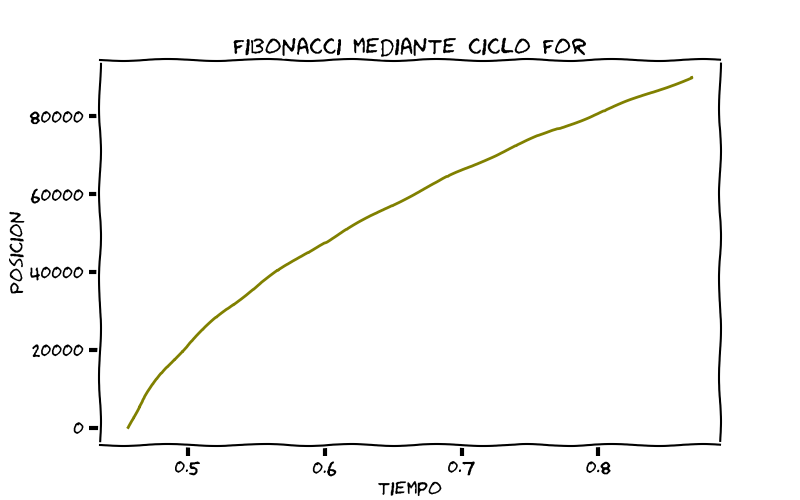
\includegraphics[width=9cm]{for.png}
\caption{gráfica for, \href{https://github.com/joescalona/Programacion-Astronomica/blob/master/Tarea\%205/Graficas/for.py}{ código aquí}} \label{figura1}
\end{minipage}
\hspace{0.5cm} % Si queremos tener un poco de espacio entre las dos figuras
\begin{minipage}[b]{0.5\linewidth}
\centering
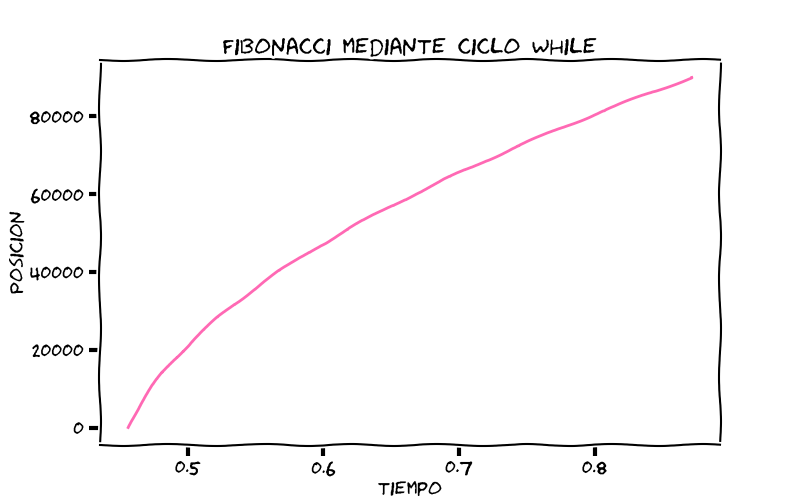
\includegraphics[width=9cm]{while.png}
\caption{gráfica while,\href{https://github.com/joescalona/Programacion-Astronomica/blob/master/Tarea\%205/Graficas/whilefib.py}{ código aquí}} \label{figura2}
\end{minipage}
\end{figure}

\begin{figure}[H] 
\begin{minipage}[b]{0.5\linewidth} %Una minipágina que cubre la mitad de la página
\centering
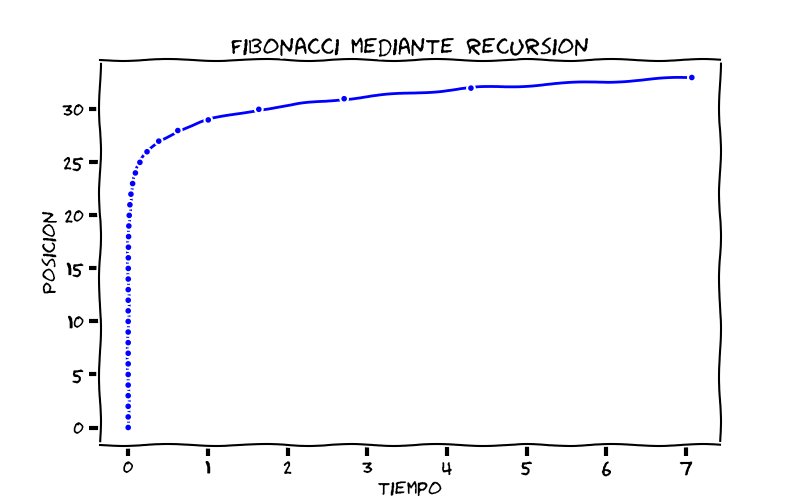
\includegraphics[width=9cm]{recursion.png}
\caption{gráfica recursion, \href{https://github.com/joescalona/Programacion-Astronomica/blob/master/Tarea\%205/Graficas/recursionfib.py}{ código aquí} } \label{figura1}
\end{minipage}
\hspace{0.5cm} % Si queremos tener un poco de espacio entre las dos figuras
\begin{minipage}[b]{0.5\linewidth}
\centering
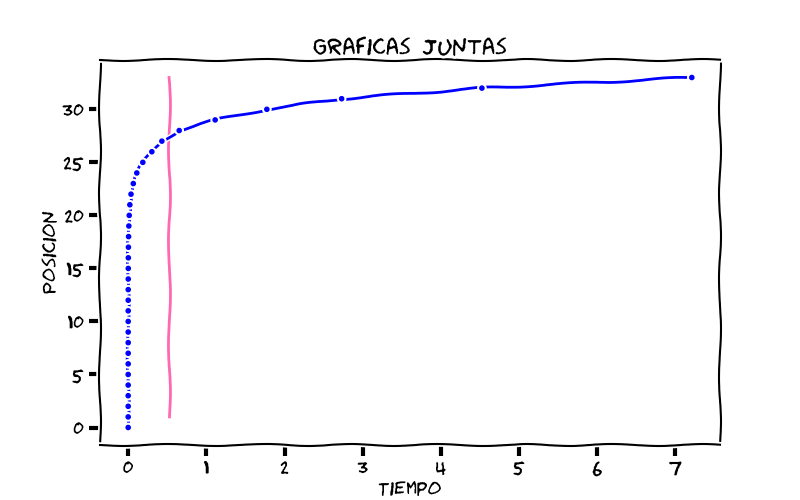
\includegraphics[width=9cm]{todos.png}
\caption{graficas juntas, \href{https://github.com/joescalona/Programacion-Astronomica/blob/master/Tarea\%205/Graficas/juntos.py}{ código aquí}} \label{figura2}
\end{minipage}
\end{figure}

No quise incluir el código en el pdf porque estaba resultando demasiado largo (sólo por tema de estética,pero lo enlacé en el link). Tanto las gráficas \textbf{for} y  \textbf{while} son aproximadamente lineales, lo cual tiene sentido ya que si uno le exige Fib(numero alto) se demorará cada vez más. La gŕafica de la función \textbf{recursiva} me resultó curiosa, se va creando una especie de asíntota desde la posición de fibonacci $\approx 34$, al ingresar Fib(35) el programa se demora mucho en calcular el número. Cabe hacer notar que los programas \textbf{for} y \textbf{while} en cada iteración entregaba el siguiente número de fibonacci. Es por esto que el eje vertical es llamado \textbf{Posición} (pero sería equivalente a Iteración) Esto no ocurre en el gráfico de \textbf{recursión} ya que no se me ocurrió la forma de contar las iteraciones dentro de la función recursiva. 
%-------------------------------------------------------------------------%

%-------------------------------------------------------------------------%
%-------------------------------------------------------------------------%


%-------------------------------------------------------------------------%
\newpage
\section{Ejercicio 6}
Escriban un código que imprima las primeras N filas (donde N ~ 10) del triángulo
de Pascal. Den el código y el output en el PDF de la tarea.

\subsection{Solución}

Para realizar este ejercicio, tuve que recurrir a youtube ya que no sabía ni siquiera cómo empezar. En mi búsqueda me topé con este \href{https://www.youtube.com/watch?v=qRnmis3nYLI&t=106s}{video} en el cual se explica (desde 0:17 hasta el min 2:09) la idea expuesta aquí. Además me fue de mucha ayuda este otro \href {https://www.youtube.com/watch?v=Ut5AGIMkPoQ}{video}

De \href{https://es.wikipedia.org/wiki/Tri\%C3\%A1ngulo_de_Pascal}{Wikipedia} cito lo siguiente: 

\textit{"La construcción del triángulo está relacionada con los coeficientes binomiales según la fórmula(también llamada regla de Pascal" \textbf{combinatoria}}
\begin{equation*}
    {n \choose k } = \frac{n!}{k!\, (n-k)!}
\end{equation*}
Código Python \href{https://github.com/joescalona/Programacion-Astronomica/blob/master/Tarea\%205/problema6.py}{aquí}
    \begin{minted}{python}
    #-*-coding: utf-8-*-
    from math import factorial
    
    print "******** TRIANGULO DE PASCAL ********"
    #se pide el número de filas
    f = abs(int(input('Ingresa el número de filas = ')))
    
    n = 0
    k = 0
    
    #comienza un ciclo dentro del otro
    while (n<=f):
        print ''
        while (k<=n):
            #numerador = n!
            num = factorial(n)
            # denominador = k! * (n-k)!
            den = (factorial(k)) * (factorial(n-k))
            #respuesta
            res = (num)/(den)
            #k aumentará para continuar con el ciclo
            #k aumentará hasta que se iguale con n 
            k = k+1
            #imprimir respuesta
            print res,#
        #variar n para continuar hasta la cantidad de filas  
        n=n+1
        #reiniciar k 
        k=0
    \end{minted}
    
    \noindent
Para N \approx 10 
    
    \begin{lstlisting}[style=C,numbers=none]
    ******** TRIANGULO DE PASCAL ********
    Ingresa el numero de filas = 10

    1 
    1 1 
    1 2 1 
    1 3 3 1 
    1 4 6 4 1 
    1 5 10 10 5 1 
    1 6 15 20 15 6 1 
    1 7 21 35 35 21 7 1 
    1 8 28 56 70 56 28 8 1 
    1 9 36 84 126 126 84 36 9 1 
    1 10 45 120 210 252 210 120 45 10 1
    
    \end{lstlisting}
%-------------------------------------------------------------------------%
%-------------------------------------------------------------------------%

\end{document}
